% !TeX root = construct.tex

\chapter{Help, My Compass Collapsed!}\label{c.collapse}

\section{Fixed compasses and collapsing compasses}

In a modern compass used for geometric constructions the distance between the two legs can be fixed so that it is possible to copy a line segment or a circle from one position to another. We will call such a compass a \emph{fixed compass}. I have seen geometry textbooks that present the  construction a perpendicular bisector to a line segment as follows: construct two circles centered at the ends of the line segment such that the radii are equal and \emph{greater than half the length of the segment} (left diagram):

\vspace{-3ex}

\begin{center}
\begin{tikzpicture}[scale=0.5]
\begin{scope}
\coordinate (A) at (0,0);
\coordinate (B) at (4,0);
\draw (A) node[below left] {$A$} -- (B) node[below right] {$B$};
\fill (A) circle[radius=3pt];
\fill (B) circle[radius=3pt];
\draw[name path=larc] (A) ++(-60:3cm) arc (-60:60:3cm);
\draw[name path=rarc] (B) ++(-120:3cm) arc (-120:-240:3cm);
\path [name intersections={of=larc and rarc,by={b,t}}];
\fill (t) node[above right,xshift=-2pt,yshift=5pt] {$C$} circle[radius=3pt];
\fill (b) node[below left,xshift=2pt,yshift=-5pt] {$D$} circle[radius=3pt];
\draw ($ (b) ! 1.2 ! (t)$) -- ($ (t) ! 1.2 ! (b)$);
\end{scope}
\begin{scope}[xshift=12cm]
\coordinate (A) at (0,0);
\coordinate (B) at (4,0);
\draw (A) node[below left] {$A$} -- (B) node[below right] {$B$};
\fill (A) circle[radius=3pt];
\fill (B) circle[radius=3pt];
\draw[name path=larc] (A) ++(-80:4cm) arc (-80:80:4cm);
\draw[name path=rarc] (B) ++(-100:4cm) arc (-100:-260:4cm);
\path [name intersections={of=larc and rarc,by={b,t}}];
\fill (t) node[above right,xshift=-2pt,yshift=3pt] {$C$} circle[radius=3pt];
\fill (b) node[below left,xshift=2pt,yshift=-3pt] {$D$}circle[radius=3pt];
\draw ($ (b) ! 1.2 ! (t)$) -- ($ (t) ! 1.2 ! (b)$);
\end{scope}
\end{tikzpicture}
\end{center}

\vspace{-3ex}

Euclid used a \emph{collapsing compass} whose legs fold up when the compass is lifted off the paper. Teachers often use a collapsing compass consisting of a piece of chalk tied to a string. It is impossible to maintain a fixed radius when the chalk is removed from the blackboard. The right diagram above shows how to construct a perpendicular bisector with a collapsing compass: the length of the segment $AB$ is, of course, equal to the length of the segment $BA$, so the radii of the two circles are equal.

The proof that the line constructed is the perpendicular bisector is not at all elementary because relatively advanced concepts like congruent triangles have to be used. However, the proof that the same construction results in an equilateral triangle is very simple (right diagram below). The length of $AC$ equals the length of $AB$ since they are radii of the same circle, and for the same reason the length of $BC$ is equal to the length of $BA$. We have:
\[
AC=AB=BA=BC\,.
\]

\begin{center}
\begin{tikzpicture}[scale=0.5]
\begin{scope}
\coordinate (A) at (0,0);
\coordinate (B) at (4,0);
\draw (A) node[below left] {$A$} -- (B) node[below right] {$B$};
\fill (A) circle[radius=3pt];
\fill (B) circle[radius=3pt];
\draw[name path=larc] (A) ++(-60:3cm) arc (-60:60:3cm);
\draw[name path=rarc] (B) ++(-120:3cm) arc (-120:-240:3cm);
\path [name intersections={of=larc and rarc,by={b,t}}];
\fill (t) node[above right,xshift=-2pt,yshift=5pt] {$C$} circle[radius=3pt];
\fill (b) node[below left,xshift=2pt,yshift=-5pt] {$D$} circle[radius=3pt];
\draw (A) -- (t);
\draw (B) -- (t);
\end{scope}
\begin{scope}[xshift=12cm]
\coordinate (A) at (0,0);
\coordinate (B) at (4,0);
\draw (A) node[below left] {$A$} -- (B) node[below right] {$B$};
\fill (A) circle[radius=3pt];
\fill (B) circle[radius=3pt];
\draw[name path=larc] (A) ++(-80:4cm) arc (-80:80:4cm);
\draw[name path=rarc] (B) ++(-100:4cm) arc (-100:-260:4cm);
\path [name intersections={of=larc and rarc,by={b,t}}];
\fill (t) node[above right,xshift=-2pt,yshift=3pt] {$C$} circle[radius=3pt];
\fill (b) node[below left,xshift=2pt,yshift=-3pt] {$D$}circle[radius=3pt];
\draw (A) -- (t);
\draw (B) -- (t);
\end{scope}
\end{tikzpicture}
\end{center}

The left diagram above shows that for the construction with the fixed compass the triangle will be isosceles, but not necessarily equilateral.

This construction of an equilateral triangle is the first proposition in Euclid's \emph{Elements}. The second proposition shows how to copy a given line segment $AB$ to a segment of the same length, one of whose end points is a given point $C$. Therefore, a fixed compass adds no additional capability. Toussaint \cite{toussaint} showed that many incorrect constructions for this proposition have been given. In fact, it was Euclid who gave a correct construction! The following section presents Euclid's construction and the proof of its correctness. Then I show an incorrect construction that can be found even in modern textbooks.

\section{Euclid's construction for copying a line segment}

\textbf{Theorem:} Given a line segment $AB$ and a point $C$, a line segment can be constructed (using a collapsing compass) at $C$ whose length is equal to the length of $AB$:

\vspace{-2ex}

\begin{center}
\begin{tikzpicture}[scale=0.4]
\begin{scope}
\coordinate (C) at (0,0);
\coordinate (A) at (2.5,0);
\coordinate (B) at (5.5,2);
\draw (A) node[below,xshift=-2pt,yshift=-2pt] {$A$} -- (B) node[right] {$B$};
\fill (A) circle[radius=3pt];
\fill (B) circle[radius=3pt];
\fill (C) node[below,xshift=2pt,yshift=-2pt] {$C$} circle[radius=3pt];
\end{scope}
\begin{scope}[xshift=12cm]
\coordinate (C) at (0,0);
\coordinate (A) at (2.5,0);
\coordinate (B) at (5.5,2);
\draw (A) node[below,xshift=-2pt,yshift=-2pt] {$A$} -- (B) node[right] {$B$};
\fill (A) circle[radius=3pt];
\fill (B) circle[radius=3pt];
\fill (C) node[below,xshift=2pt,yshift=-2pt] {$C$} circle[radius=3pt];
\draw (A) -- (C);
\path[name path=larc] (C) ++(-70:2.5cm) arc (-70:70:2.5cm);
\path[name path=rarc] (A) ++(-110:2.5cm) arc (-110:-250:2.5cm);
\path [name intersections={of=larc and rarc,by={d,D}}];
\fill (D) node[above] {$D$} circle[radius=3pt];
\draw (A) -- (D);
\draw (C) -- (D);
\end{scope}
\end{tikzpicture}
\end{center}

\vspace{-2ex}

\textbf{Construction:}

Construct the line segment from $A$ to $C$.

Construct an equilateral triangle whose base is $AC$ (right diagram above). Label the third vertex $D$. By Euclid's first proposition, the triangle can be constructed using a collapsing compass.

Construct a ray that is a continuation of $DA$ and a ray that is a continuation of $DC$ (left diagram below).

Construct a circle centered at $A$ with radius $AB$. Label the intersection of the circle and the ray $DA$ by $E$ (right diagram below).

\begin{center}
\begin{tikzpicture}[scale=0.4]
\begin{scope}
\coordinate (C) at (0,0);
\coordinate (A) at (2.5,0);
\coordinate (B) at (5.5,2);
\draw (A) node[below,xshift=-2pt,yshift=-2pt] {$A$} -- (B) node[right] {$B$};
\fill (A) circle[radius=3pt];
\fill (B) circle[radius=3pt];
\fill (C) node[below,xshift=2pt,yshift=-2pt] {$C$} circle[radius=3pt];
\draw (A) -- (C);
\path[name path=larc] (C) ++(-70:2.5cm) arc (-70:70:2.5cm);
\path[name path=rarc] (A) ++(-110:2.5cm) arc (-110:-250:2.5cm);
\path [name intersections={of=larc and rarc,by={d,D}}];
\fill (D) node[above] {$D$} circle[radius=3pt];
\draw (A) -- (D);
\draw (C) -- (D);
\draw[name path=ray2] (D) -- ($ (D) ! 3 ! (C) $);
\draw[name path=ray1] (D) -- ($ (D) ! 3 ! (A) $);
\end{scope}
\begin{scope}[xshift=12cm]
\coordinate (C) at (0,0);
\coordinate (A) at (2.5,0);
\coordinate (B) at (5.5,2);
\draw (A) node[below,xshift=-2pt,yshift=-2pt] {$A$} -- (B) node[right] {$B$};
\fill (A) circle[radius=3pt];
\fill (B) circle[radius=3pt];
\fill (C) node[below,xshift=2pt,yshift=-2pt] {$C$} circle[radius=3pt];
\draw (A) -- (C);
\path[name path=larc] (C) ++(-70:2.5cm) arc (-70:70:2.5cm);
\path[name path=rarc] (A) ++(-110:2.5cm) arc (-110:-250:2.5cm);
\path [name intersections={of=larc and rarc,by={d,D}}];
\fill (D) node[above] {$D$} circle[radius=3pt];
\draw (A) -- (D);
\draw (C) -- (D);
\draw[name path=ray2] (D) -- ($ (D) ! 3 ! (C) $);
\draw[name path=ray1] (D) -- ($ (D) ! 3 ! (A) $);
\node[draw,circle through=(B),name path=c1] at (A) {};
\path [name intersections={of=c1 and ray1,by={E,e}}];
\fill (E) node[right,xshift=2pt,yshift=-2pt] {$E$} circle[radius=3pt];
\end{scope}
\end{tikzpicture}
\end{center}

Construct a circle centered at $D$ with radius $DE$. Label the intersection of the circle and the ray $DC$ by $F$:

\vspace*{-2ex}

\begin{center}
\begin{tikzpicture}[scale=0.4]
\coordinate (C) at (0,0);
\coordinate (A) at (2.5,0);
\coordinate (B) at (5.5,2);
\draw (A) node[below,xshift=-2pt,yshift=-2pt] {$A$} -- node[above] {$x$} (B) node[right] {$B$};
\fill (A) circle[radius=3pt];
\fill (B) circle[radius=3pt];
\fill (C) node[below,xshift=2pt,yshift=-2pt] {$C$} circle[radius=3pt];
\draw (A) -- (C);
\path[name path=larc] (C) ++(-70:2.5cm) arc (-70:70:2.5cm);
\path[name path=rarc] (A) ++(-110:2.5cm) arc (-110:-250:2.5cm);
\path [name intersections={of=larc and rarc,by={d,D}}];
\fill (D) node[above] {$D$} circle[radius=3pt];
\draw (A) -- node[right] {$y$} (D);
\draw (C) -- node[left] {$y$} (D);
\draw[name path=ray2] (D) -- ($ (D) ! 3 ! (C) $);
\draw[name path=ray1] (D) -- ($ (D) ! 3 ! (A) $);
\node[draw,circle through=(B),name path=c1] at (A) {};
\path [name intersections={of=c1 and ray1,by={E,e}}];
\fill (E) node[right,xshift=2pt,yshift=-2pt] {$E$} circle[radius=3pt];
\node[draw,circle through=(E),name path=c2] at (D) {};
\path [name intersections={of=c2 and ray2,by={F,f}}];
\fill (F) node[left,xshift=-2pt,yshift=-2pt] {$F$} circle[radius=3pt];
\path (A) -- node[right] {$x$} (E);
\path (C) -- node[left] {$x$} (F);
\end{tikzpicture}
\end{center}

\vspace*{-1ex}

\textbf{Claim:} The length of the line segment $CF$ is equal to the length of $AB$.

\textbf{Proof:} $DC=DA$ because $\triangle ACD$ is equilateral. $AE=AB$ because they are radii of the same circle centered at $A$. $DF=DE$ because they are radii of the same circle centered at $D$. Therefore, the length of the line segment $CF$ is:

\vspace*{-1ex}

\[
CF=DF-DC=DE-DC=DE-DA=AE=AB\,.
\]


\vspace*{-1ex}

%%%%%%%%%%%%%%%%%%%%%%%%%%%%%%%%%%%%%%%%%%%%%%%%%%%%%%%%%%%%%%%

\section{An incorrect construction for copying a line segment}\label{s.erroneous}

\textbf{Construction(\cite{rusty}):}

Construct a circle centered at $A$ with radius $AB$:

\begin{center}
\begin{tikzpicture}[scale=0.4]
\begin{scope}
\coordinate (C) at (-2,0);
\coordinate (A) at (2.5,0);
\coordinate (B) at (4.5,1.5);
\draw (A) node[below,xshift=-2pt,yshift=-2pt] {$A$} -- (B) node[right] {$B$};
\fill (A) circle[radius=3pt];
\fill (B) circle[radius=3pt];
\fill (C) node[below,xshift=2pt,yshift=-2pt] {$C$} circle[radius=3pt];
\end{scope}
\begin{scope}[xshift=12cm]
\coordinate (C) at (-2,0);
\coordinate (A) at (2.5,0);
\coordinate (B) at (4.5,1.5);
\draw (A) node[below,xshift=-2pt,yshift=-2pt] {$A$} -- (B) node[right] {$B$};
\fill (A) circle[radius=3pt];
\fill (B) circle[radius=3pt];
\fill (C) node[below,xshift=2pt,yshift=-2pt] {$C$} circle[radius=3pt];
\node[draw,circle through=(B),name path=c1] at (A) {};
\end{scope}
\end{tikzpicture}
\end{center}

Construct a circle centered at $A$ with radius $AC$ and a circle centered at $C$ with radius $AC=CA$. Label the intersections of the two circles $E,F$. Label the intersection of the circle centered at $C$ and the circle centered at $A$ with radius $AB$ by $D$:

\begin{center}
\begin{tikzpicture}[scale=0.5]
\coordinate (C) at (-2,0);
\coordinate (A) at (2.5,0);
\coordinate (B) at (4.5,1.5);
\draw (A) node[below right] {$A$} -- (B) node[right] {$B$};
\fill (A) circle[radius=3pt];
\fill (B) circle[radius=3pt];
\fill (C) node[left,xshift=-2pt] {$C$} circle[radius=3pt];
\node[draw,circle through=(B),name path=c1] at (A) {};
\node[draw,circle through=(C),name path=c2] at (A) {};
\node[draw,circle through=(A),name path=c3] at (C) {};
\path [name intersections={of=c1 and c3,by={D,f}}];
\path [name intersections={of=c2 and c3,by={E,F}}];
\fill (D) node[below right,xshift=4pt] {$D$} circle[radius=3pt];
\fill (E) node[above,yshift=2pt] {$E$} circle[radius=3pt];
\fill (F) node[below,yshift=-2pt] {$F$} circle[radius=3pt];
\end{tikzpicture}
\end{center}

Construct a circle centered at $E$ with radius $ED$. Label the intersection of this circle with the circle centered at $A$ with radius $AC$ by $G$:

\begin{center}
\begin{tikzpicture}[scale=0.5]
\coordinate (C) at (-2,0);
\coordinate (A) at (2.5,0);
\coordinate (B) at (4.5,1.5);
\draw (A) node[below right] {$A$} -- (B) node[right] {$B$};
\fill (A) circle[radius=3pt];
\fill (B) circle[radius=3pt];
\fill (C) node[below left] {$C$} circle[radius=3pt];
\node[draw,circle through=(B),name path=c1] at (A) {};
\node[draw,circle through=(C),name path=c2] at (A) {};
\node[draw,circle through=(A),name path=c3] at (C) {};
\path [name intersections={of=c1 and c3,by={D,f}}];
\path [name intersections={of=c2 and c3,by={E,F}}];
\fill (D) node[below right,xshift=4pt] {$D$} circle[radius=3pt];
\fill (E) node[above,yshift=2pt] {$E$} circle[radius=3pt];
\fill (F) node[below,yshift=-2pt] {$F$} circle[radius=3pt];
\node[draw,circle through=(D),name path=c4] at (E) {};
\path [name intersections={of=c2 and c4,by={g,G}}];
\fill (G) node[below left,xshift=-4pt] {$G$} circle[radius=3pt];
\draw (C) -- (G);
\draw[dashed] (G) -- (E) -- (C);
\draw[dashed] (A) -- (D) -- (E) -- cycle;
\end{tikzpicture}
\end{center}

\textbf{Claim:} The length of the line segment $GC$ is equal to the length of $AB$.

\textbf{Proof:} We shall show that $\triangle ADE\cong\triangle CGE$. If so, $CG=AD=AB$ because $AB,AD$ are radii of the smaller circle centered at $A$. The circle centered at $C$ has the same radius as the circle centered at $A$ that goes through $E$, so we can consider that they are the ``same'' circle.

$EG=ED$ because they are radii of the circle centered at $E$ and $EC=EA$ because they are radii of the ``same'' circle. $\angle GCE=\angle DAE$ because they are central angles that intercept the ``same'' chord and $\angle CGE=\angle ADE$ because they are inscribed angles intercepting the ``same'' chord. Therefore, $\angle GEC=\angle DEA$ and $\triangle GEC\cong \triangle DAE$ by SAS. 

The answer: there isn't any error in the proof! The problem arises from a different source: the equality $AB=GC$ holds only when the length of $AB$ is less that the length of $AC$. In contrast, Euclid's construction and proof are true, independent of the relative lengths of  $AB$ and $AC$, and of the position of the point $C$ relative to the line segment $AB$ (\cite{toussaint}).


%%%%%%%%%%%%%%%%%%%%%%%%%%%%%%%%%%%%%%%%%%%%%%%%%%%%%%%%%%%%%%%

\section{A ``simpler'' construction for copying a line segment}

Given a line segment $AB$ and a point $C$, if we can build a parallelogram with these three points as its vertices, we obtain a line segment with $C$ at one end whose length is equal to the length of $AB$ (left diagram left):
\begin{center}
\begin{tikzpicture}[scale=0.7]
\coordinate (A) at (0,0);
\coordinate (B) at (4,0);
\coordinate (C) at (5,2);
\draw (A) -- (B);
\path (A) -- node[above] {$x$} (B);
\fill (A) node[below left] {$A$} circle[radius=3pt];
\fill (B) node[below] {$B$} circle[radius=3pt];
\fill (C) node[above] {$C$} circle[radius=3pt];
\draw (B) -- node[right] {$y$} (C);
\coordinate (D) at ($(C)+(-40mm,0cm)$);
\draw (D) -- node[above] {$x$} (C);
\draw (A) -- node[left] {$y$} (D);
\fill (D) node[above] {$D$} circle[radius=3pt];
\begin{scope}[xshift=12cm]
\coordinate (A) at (0,0);
\coordinate (B) at (4,0);
\coordinate (C) at (5,2);
\draw ($ (B) ! 1.2 ! (A) $) -- ($ (A) ! 1.5 ! (B) $);
\path (A) -- (B);
\fill (A) node[below left,xshift=-4pt] {$A$} circle[radius=3pt];
\fill (B) node[below] {$B$} circle[radius=3pt];
\fill (C) node[above] {$C$} circle[radius=3pt];
\draw (B) -- (C);
\draw[name path=ray1] ($(C)+(-5cm,0cm)$) -- ($(C)+(1cm,0cm)$);
\draw[name path=ray2] ($(A)+(-.25,-.65)$) -- ($(A)+(1,2.6)$);
\path [name intersections={of=ray1 and ray2,by={D}}];
\fill (D) node[above left] {$D$} circle[radius=3pt];
\coordinate (E) at (C |- B);
\draw[thick,dashed] (C) -- (E);
\fill (E) node[below] {$E$} circle[radius=3pt];
\draw[rotate=-90] (C) rectangle +(10pt,10pt);
\draw (E) rectangle +(10pt,10pt);
\coordinate (F) at ($(A)!(B)!(D)$);
\fill (F) circle[radius=3pt];
\draw[thick,dashed] (B) -- (F);
\draw[rotate=-24] (F) rectangle +(10pt,10pt);
\draw[rotate=67] (B) rectangle +(10pt,10pt);
\end{scope}
\end{tikzpicture}
\end{center}
This construction can be found in \cite[pp. 207--208]{roads}.

\textbf{Construction (right diagram):}

Construct the line segment from $B$ to $C$.

Construct an altitude from $C$ to the line containing the line segment $AB$. Label the intersection by $D$.

Construct an altitude to the line segment $CD$ at $C$. This line is parallel to $AB$.

Use a similar method to construct a line parallel to $BC$ through $A$. Label the intersection of the two lines by $D$.

$AD\|BC$, $AB\|DC$ and by definition $ABCD$ is a parallelogram, so $AB=CD$ as required.

\textbf{Construction with a collapsing compass:} We will show that it is possible to construct an altitude through a given point with a collapsing compass. Construct a circle centered at $C$ with a radius that is greater than the distance of $C$ from the line. Label the intersections with the line by $D,E$. Construct circles centered at $D,E$ with radii $DC=EC$:
\begin{center}
\begin{tikzpicture}[scale=0.5]
\coordinate (A) at (0,0);
\coordinate (B) at (4,0);
\coordinate (C) at (5,2);
\draw[name path=ray] ($ (B) ! 1.5 ! (A) $) -- ($ (A) ! 2.5 ! (B) $);
%\fill (A) node[below] {$A$} circle[radius=3pt];
%\fill (B) node[below] {$B$} circle[radius=3pt];
\fill (C) node[right] {$C$} circle[radius=3pt];
\draw[name path=arc] (C) ++(-160:3.5cm) arc (-160:-20:3.5cm);
\path [name intersections={of=arc and ray,by={D,E}}];
\fill (D) node[below left] {$D$} circle[radius=3pt];
\fill (E) node[below right] {$E$} circle[radius=3pt];
\draw[name path=larc] (D) ++(-60:3.5cm) arc (-60:60:3.5cm);
\draw[name path=rarc] (E) ++(-120:3.5cm) arc (-120:-240:3.5cm);
\path [name intersections={of=larc and rarc,by={b,t}}];
\fill (b) node[right] {$F$} circle[radius=3pt];
\draw ($ (b) ! 1.2 ! (t)$) -- ($ (t) ! 1.2 ! (b)$);
\end{tikzpicture}
\end{center}
The line connecting the intersections of the circles $C,F$ is an altitude through $C$.

The proof the correctness of this construction is much more difficult than Euclid's proof of his construction.

%%%%%%%%%%%%%%%%%%%%%%%%%%%%%%%%%%%%%%%%%%%%%%%%%%%%%%%%%%%%%%%

\section{Don't trust a diagram}

In Section~\ref{s.erroneous}, we saw that a diagram can lead us astray. Here is a proof that \emph{all} triangles are isosceles!
\begin{center}
\begin{tikzpicture}[scale=1.1]
\coordinate (P) at (0,0);
\node[xshift=4mm,yshift=1mm] at (P) {$P$};
\coordinate [label=left:$B$] (B)  at (-2,-2);
\coordinate [label=right:$C$] (C)  at (4,-2);
\coordinate [label=above:$A$] (A)  at (-1,2);
\node[below,yshift=-12pt,xshift=2pt] at (A) {$\alpha$};
\node[below,yshift=-12pt,xshift=15pt] at (A) {$\alpha$};
\draw (A) -- (B);
\draw (A) -- (C);
\draw (B) -- (C);
\draw (A) -- (P);
\draw (B) -- (P);
\draw (C) -- (P);
\coordinate[label=left:$E$] (E) at ($ (A) ! .44 ! (B) $);
\draw[rotate=-100] (E) rectangle +(4pt,4pt);
\draw (P) -- (E);
\coordinate (F) at ($ (A) ! .33 ! (C) $);
\node[right,xshift=2pt,yshift=2pt] at (F) {$F$};
\draw[rotate=-132] (F) rectangle +(4pt,4pt);
\draw (P) -- (F);
\coordinate[label=below:$D$] (D) at ($ (B) ! .33 ! (C) $);
\draw (D) rectangle +(4pt,4pt);
\draw (P) -- (D);
\node[left] at ($ (A) ! .5 ! (E) $) {};
\node[left] at ($ (B) ! .5 ! (E) $) {};
\node[below] at ($ (B) ! .5 ! (D) $) {$a$};
\node[below] at ($ (C) ! .5 ! (D) $) {$a$};
\node[right,xshift=2pt] at ($ (A) ! .5 ! (F) $) {};
\node[right,xshift=2pt] at ($ (C) ! .5 ! (F) $) {};
\foreach \n in {A,B,C,D,E,F,P} {
  \fill (\n) circle[radius=1pt];
}
\end{tikzpicture}
\end{center}
Given an arbitrary triangle $\triangle ABC$, let $P$ be the intersection of the angle bisector of $\angle BAC$ and the perpendicular bisector $BC$. Label by $D,E,F$ the intersections of the altitudes from $P$ to the sides $BC, AB,AC$. $\triangle APF\cong \triangle APE$ because they are right triangles with equal angles $\alpha$ and a common side $AP$.

$\triangle DPC\cong \triangle DPB$ SAS because $PD$ is a common side, $\angle PDB=\angle PDC=90$ and $BD=DC=a$ because $PD$ is the perpendicular bisector of $BC$. $\triangle EPB\cong \triangle EPC$ because $EP=PF$ by the first congruence and $PB=PC$ by the second congruence. By combining the equations we get that $\triangle ABC$ is isoceles:
\[
AB= AE+EB=AF+FC =AC\,.
\]
The problem with the proof is that the diagram is incorrect because point $P$ is \emph{outside} the triangle, as can be seen from the following diagram constructed using GeoGebra:
\begin{center}
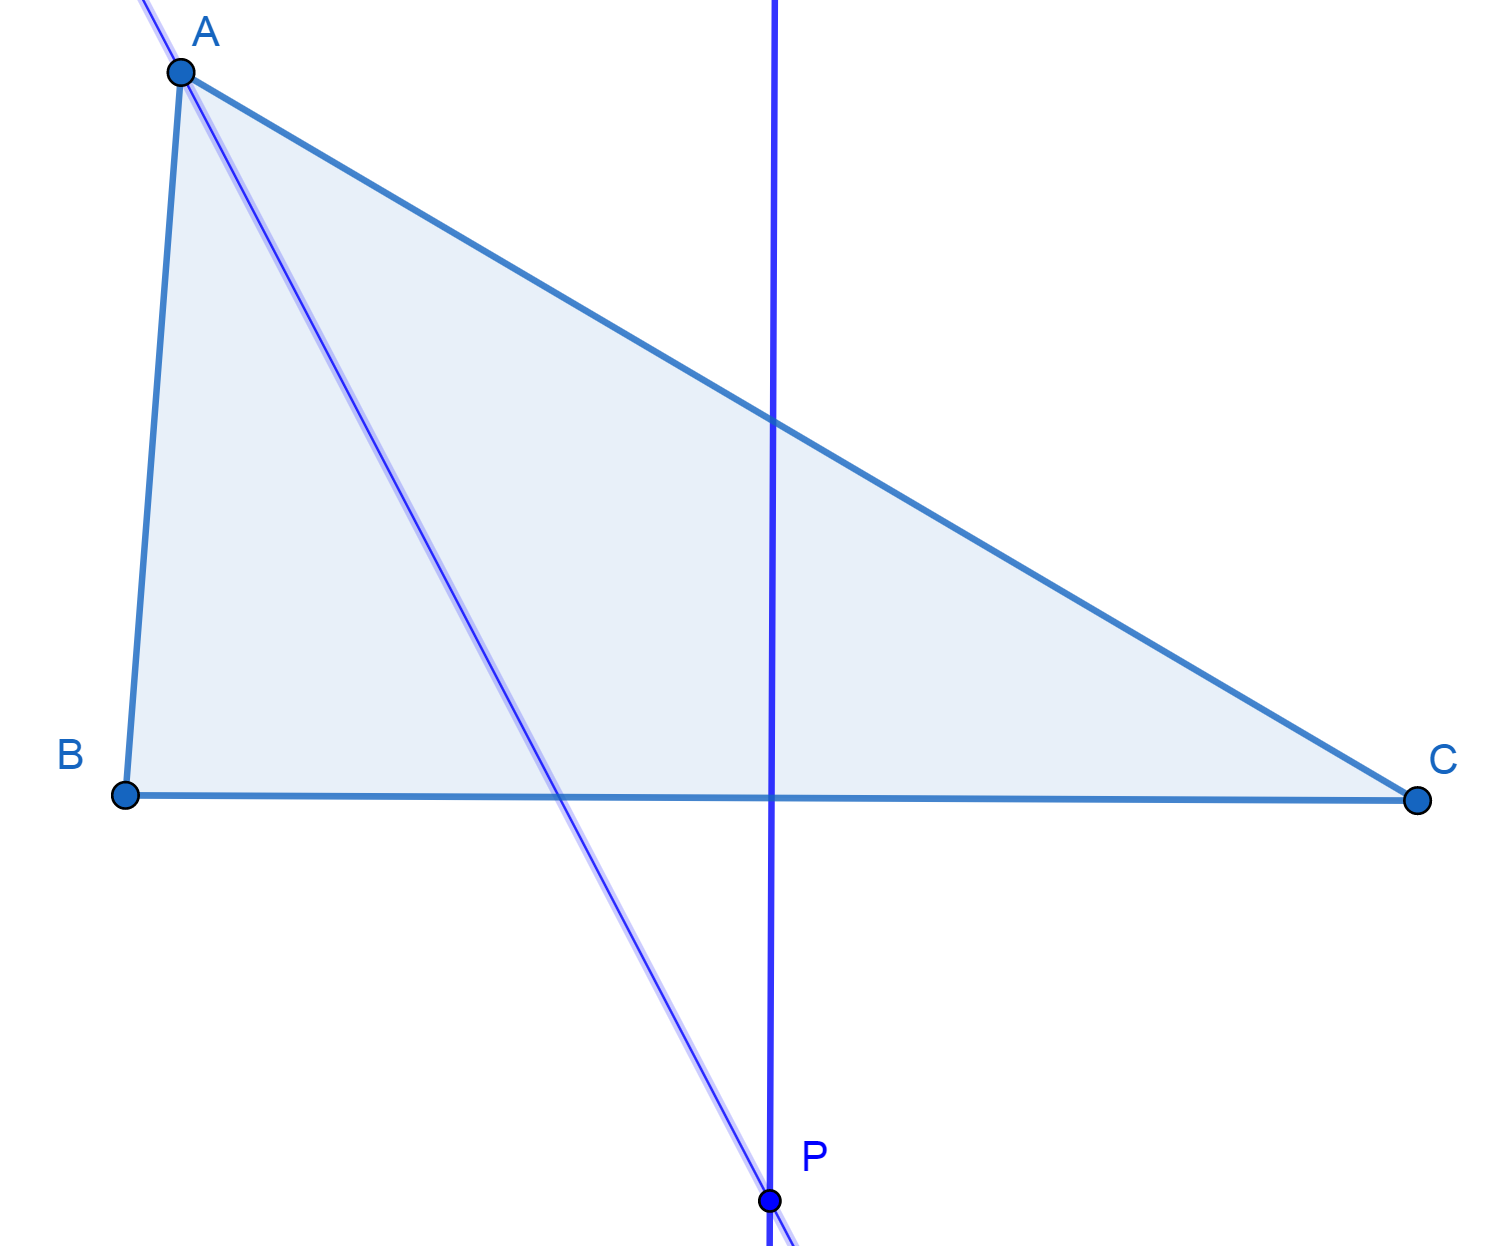
\includegraphics[width=.5\textwidth]{isoceles}
\end{center}

